\documentclass{article}
\usepackage{../fasy-hw}

%% UPDATE these variables:
\renewcommand{\hwnum}{6}
\title{Discrete Structures, Homework \hwnum}
\author{Patrick O'Connor (Patrick OConnor (322))}
\collab{n/a}
\date{due: 6 April 2021}

\begin{document}

\maketitle

This homework assignment should be
submitted as a single PDF file both to D2L and to Gradescope.

General homework expectations:
\begin{itemize}
    \item Homework should be typeset using LaTex.
    \item Answers should be in complete sentences and proofread.
    \item You will not plagiarize, nor will you share your written solutions
        with classmates.
    \item List collaborators at the start of each question using the \texttt{collab} command.
    \item Put your answers where the \texttt{todo} command currently is (and
        remove the \texttt{todo}, but not the word \texttt{Answer}).
\end{itemize}


% ============================================
% ============================================
\collab{N/A} \nextprob{Applications}
% ============================================
% ============================================

The topics in this class are mathematical in nature, but have strong ties to
computer science: either for understanding how computers work, why algorithms are
correct, or for how to convert real-world data into things that can be analyzed
using a computer.  Explain how each of the following tie to computer science or
data science:

\begin{enumerate}

    \item Tree (be sure that your answer needs a tree, and not a general graph)

        \paragraph{Answer}

        Trees as a data structure are utilized in countless applications in computer
        science. Such as using a BST to organize data in order to decrease the time
        complexity of insertions and deletions of data. Along with this other variations
        of trees are useful in computer science such as heaps. Heaps are extremely useful
        when creating priority ques as many of us saw in the end of CSCI 232.

    \item Directed Graph

        \paragraph{Answer}

        Directed Graphs or digraphs are similar to the afore mentioned trees in that they are used
        in abundance in computer science. Digraphs are used by compilers although I do not know the ins and outs of this.
        Along with compilers digraphs are an excellent tool for representing network graphs
        and also road networks and therefore are useful in optimal path finding.

    \item Equivalence Classes

        \paragraph{Answer}

        Equivalence Classes are an essential component when creating and testing software
        any software. Considering equivalence classes when create test can reduce the amount of
        time spent implementing while increasing the completeness of your test when done
        correctly. An example of this is if you think that they test the same thing then it is worth
        putting them together into an equivalence class.

<<<<<<< HEAD
    \item Distance Metrics

        \paragraph{Answer}

        Although I don't have much knowledge of machine learning from the reading that I have done
        in this field I know that distance metrics are essential in determining the similarity of data-points
        that will later be turned into clusters. This distance metric is measured on vectors, which are by definition
        nonnegative. This is then used to measure relativity and then later to train models and analyze data.

=======
>>>>>>> aec57f0af969fbfa3c6ffb07def4695447979b89
    \item Injective Function

        \paragraph{Answer}

        Injective functions are when a single input will always provide the same output or mathematically
        put a one to one relationship exist between the domain and the co-domain. This can be used in
        CS when creating relational database. This database is connected to one another and requesting information
        when set up correctly will return only the information that you requested in that input.



\end{enumerate}


% ============================================
% ============================================
\collab{\todo{}} \nextprob{Distance Functions}
% ============================================
% ============================================

Suppose you maintain a database of cocktail recipes.  You want to write a
application that asks a user for their favorite cocktail and returns a cocktail
that they might like.  To do so, you define the distance between two cocktails
to be the symmetric distance between their ingredient lists.  Then, for the
input cocktail, you compute the distance to every cocktail in your database and
return one of the cocktails that minimizes this distance.

\begin{enumerate}

    \item Prove that this distance is a metric. (Note: first, formally write out
        what the distance function is, including the domain and codomain).

        \paragraph{Answer}

        \todo{your answer here}

    \item Is this a good distance to use for your application?  Why or why not?

        \paragraph{Answer}

        \todo{your answer here}

\end{enumerate}


% ============================================
% ============================================
\collab{N/A} \nextprob{Loop Invariant}
% ============================================
% ============================================

Recall that a loop invariant is used to prove that a loop is correct (which in
turn helps to prove that an algorithm is correct).

\begin{enumerate}

    \item Write pseudocode that uses a while loop to find the second largest
        element in an unsorted array.  The input to your algorithm should be an
        unsorted array $A$ of real values.  The psuedocode should use the
        variable name \textsc{curguess} to store the current guess of the second
        largest value, and \textsc{curmax} to store the current max of $A$.

        \paragraph{Answer}

        \begin{algorithm}
        	\caption{Second Largest Element}
        	\begin{algorithmic}[1]
            \State{$unsortedArrayA=[A[1],A[2],\ldotsA[n]]$}
            \State{$CURMAX=$}                     \Comment{\\$P$}
            \State{$CURGUESS=$}                   \Comment{ \\|precondition $P$}
            \State{$counter=0$}                   \Comment{\\$P$}

              \While{$counter \leq unsortedArrayA.length$} \Comment{\\loop guard $G$}
                \If {$unsortedArrayA[counter] > CURMAX$}
                  \State{$CURGUESS=CURMAX$}
                  \State{$CURMAX=A[counter]$}
                  \State{$counter++$}
                \EndIf

                \If{$unsortedArrayA[counter] > CURGUESS && unsortedArrayA[counter] < CURMAX$}
                  \State{$CURGUESS = unsortedArrayA[counter]$}
                  \State{$counter++$}
                \EndIf
              \EndWhile
              \Else
                \State \textbf{return} CURGUESS   \Comment{\\postcondition $Q$}
        	\end{algorithmic}
        \end{algorithm}

    \item What is the postcondition of the loop? (Call this statement $Q$).

        \paragraph{Answer}
        The postcondition of the loop is CURGUESS and it is an element of unsortedArrayA
        and it will return the second largest element.

    \item What is the precondition of the loop? (Call this statement $P$).

        \paragraph{Answer}

        The preconditions of the loop is CURMAX, CURGUESS, and counter=0.

    \item What is the loop guard of the loop? (Call this statement $G$).

        \paragraph{Answer}

        The loop gaurd is the inside conditional statement of $unsortedArrayA[counter] > CURMAX$

    \item Prove that the loop invariant is when entering the $i^\text{th}$
        iteration of the loop is, ``the variable \textsc{curguess} stores
        the second
        largest value of $A[1,2, \ldots, i]$,
        and \textsc{curmax} stores the largest value of $A[1,2,\ldots, i]$."

        \paragraph{Answer}

        CURMAX is the maximum and CURGUESS is the second maximum in $A[1,2,\ldots, i]$
        being I[i] and this is the induction hypothesis.

        $A[i+1] = CURMAX$

        $A[i+1]$ is greater than preceding elements and as such $CURMAX = A[i+1]$
        and among original elements $CURGUESS =$ previous max.

        Thus $CURGUESS = CURMAX$ and $CURMAX = A[i+1]$ which satisfy the condition.

        $A[i+1] > CURGUESS$ but $A[i+1] < CURMAX$.
        Therefore the largest element is still $CURMAX$. But not the update will
        change the $CURGUESS$ to the new element of $A[i+1]$.

        With this we can now state, $A[i+1] < CURGUESS$ and that for either $A[1,2,\ldots, i]$
        or $A[1,2,\ldots, i+1]$.

        Thus, $I(i+1)$ is true and the postcondition that $CURGUESS$ is the second largest
        element in Array A is fulfilled.


\end{enumerate}



% ============================================
% ============================================
\collab{N/A} \nextprob{Four Colors Suffice}
% ============================================
% ============================================

Read Chapters $9$ and $10$ of \emph{Four Colors Suffice}.

\begin{enumerate}

    \item What is a \emph{reducible configuration}?

        \paragraph{Answer}

        A reducible configuration is a configuration of countries in which the map
        can be reduced to a smaller map. This is essential for the four color
        theorem as it allows maps to be broken into smaller configurations and if this
        reduced size configuration is four colorable then there is a way to add the piece
        back and achieve four color-ability once again.



    \item Who was the first to correctly prove the four color theorem?  What
        role did computers play in the proof?

        \paragraph{Answer}

        Kenneth Appel and Wolfgang Haken were the first to correctly prove the
        four color theorem in 1976. Computers played a crucial role in determining that
        four colors would suffice. With the assistance of the work done by German Mathematician
        Heinrich Heesch on the concept of reducibility; Appel and Haken were able to determine
        an unavoidable set of reducible configurations(1,834 configurations). Along with this
        Heesch's work to use discharging was important in proving this unavoidability section.
        Although computers were essential they were used almost completely to work on reducing
        the number of configurations rather than the unavoidability that was checked by hand.



    \item Draw a ``map'' on the M\"obius strip that requires five or more colors
        to color.

        \paragraph{Answer}

        \begin{figure}
          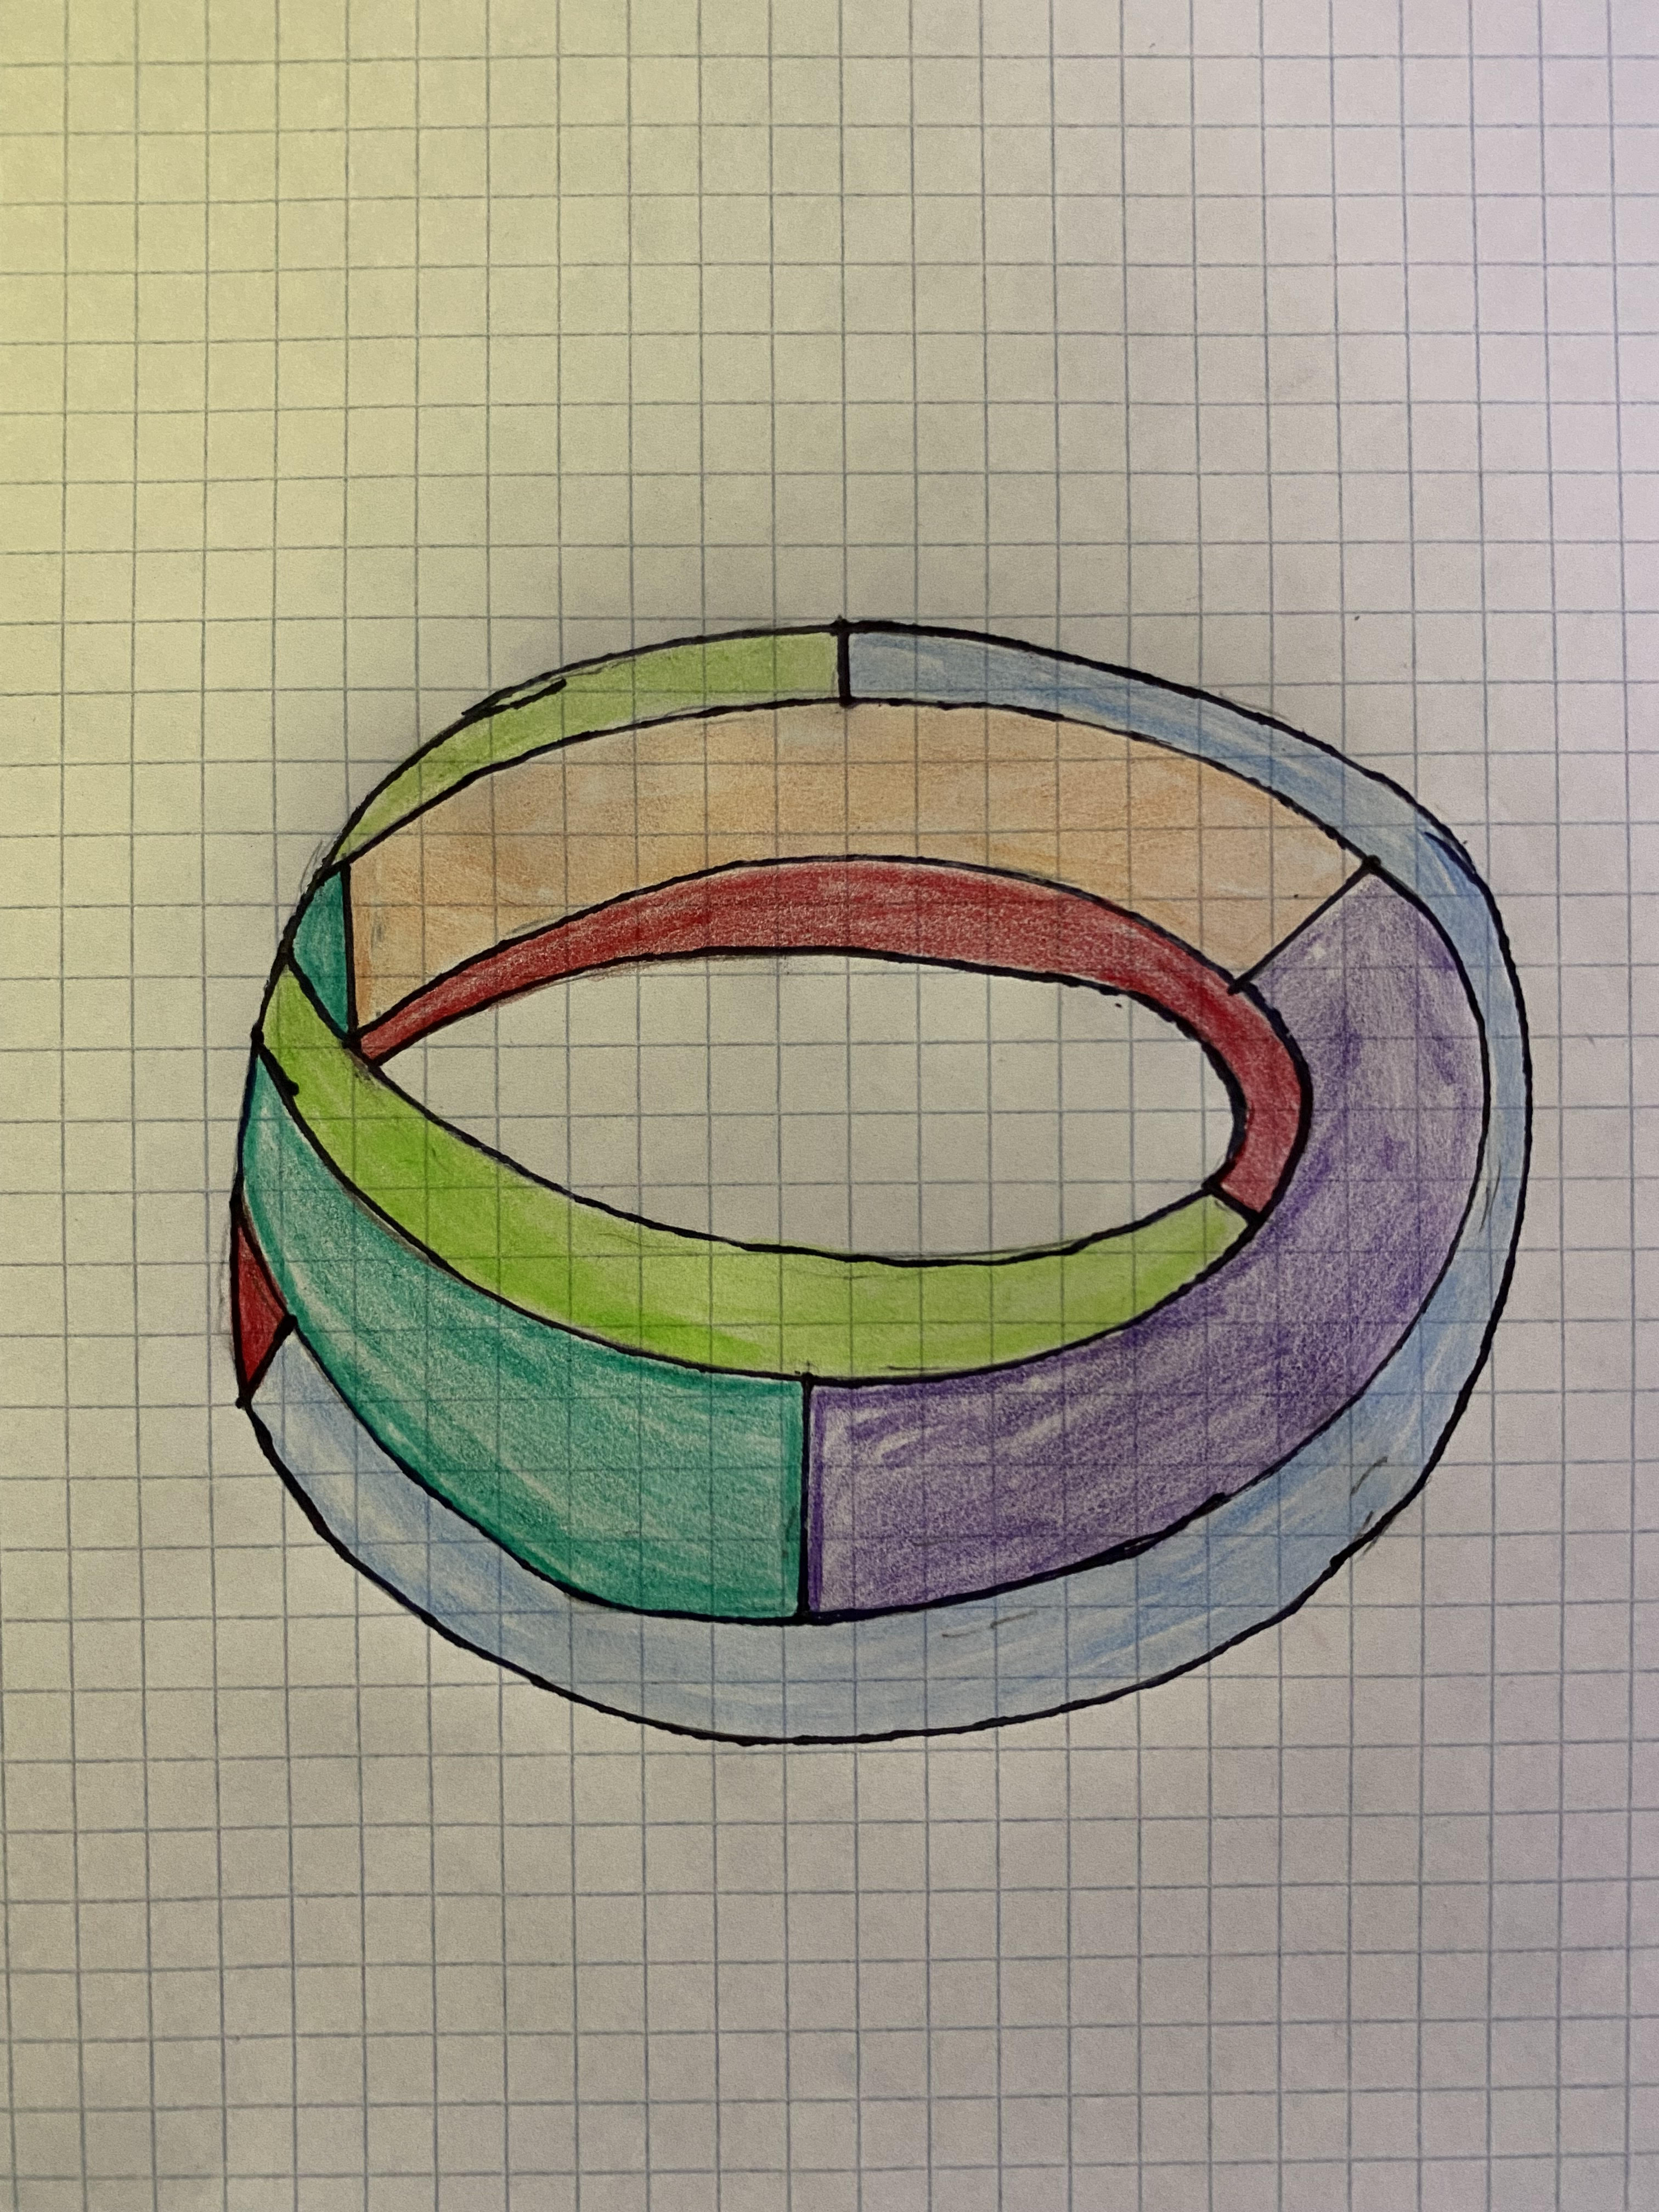
\includegraphics[width=\linewidth]{six-mobius.png}
          \caption{M\"obius strip that requires five or more colors}
          \label{fig:sixmob}
        \end{figure}
Figure \ref{fig:sixmob} Mobius strip that requires five or more colors


\end{enumerate}

% ============================================
% ============================================
\collab{N/A}
\nextprob{Shafi Goldwasser}
% ============================================
% ============================================

Write a short (1-2 paragraph) biography of Shafi Goldwasser.
\textbf{In your own words}, describe who they are and why they are important in
the history of computer science.

If you use external resources, please provide
proper citations. If you do not use external sources, please write ``I did not
use any sources to write this biography'' as the last sentence of the
biography.

\paragraph{Answer}

Shafi Goldwasser is an Israeli-American computer science who began her life in New York City in 1959.
At a young age her family moved back to Israeli where she attended grade school. Staying
in Israeli she became increasingly interested in Physics, Mathematics, and Literature.
After completing high school, Shafi returned to America to study mathematics at Carnegie Mellon University.
While studying there she discovered a love for computer science and programming. After graduating, she interned at
the RAND Corporation in LA, California. After finding lust for the California way of living, she enrolled
in graduate school at the University of California, Berkeley. There she completed a masters and doctorates in
computer science while being supervised by Manuel Blum.

After graduating, Shafi went on to MIT to do great work
in the field of computation as a professor. Dr. Goldwasser gained a keen eye and made impressive
 expansions in the areas computational complexity theory, cryptography, and computational number theory.
Within theses field Goldwasser made the largest impact in the computation area of cryptography.
Within cryptography she co-invented probabilistic encryption which is still to this day considered
the gold standard for data encryption security. Along with this she also co-invented
zero-knowledge proofs which are now used in the designing of cryptographic protocols. With an expansive
list of advancements Goldwasser and Silvio Micali were awarded a ACM A.M. Turing Award for pioneering the field
of provable security which later laid the mathematical groundwork for modern cryptography to be possible.
\emph{ACM}~\cite{acm}
\emph{Wikipedia}~\cite{wikipedia}
\emph{Berkeley Faculty}~\cite{berkeley}


% %% ... the bibliography
 \newpage
 \bibliographystyle{acm}
 \bibliography{biblio}

\end{document}
